\section{Decoding Reed--Solomon Code}
\lecture{29 Apr.}

Though the Reed--Solomon is a very strong code, it is only used in QR codes and cloud storage (secretly). As we will discuss in the next chapter, modern day wireless communication utilizes polar codes or LDPC codes. Why the difference?

For wireless communication, agents communicate via sending electromagnetic waves. One of the oldest method to encode information into the wave is by sequentially turning on and off the wave to generate pulses which the decoder can decode. A modern dat method is to encode the information into the amplitude and phase of the wave:
\begin{equation*}
    A\ee^{i\theta} \ee^{i2\pi ft}.
\end{equation*}
Each codeword will be a different complex number $A\ee^{i\theta}$ on the complex plane, forming a \textit{constellation set}.

For cloud storage, a data center contains lots of hard disk drives containing information. Sometimes a disk fails, but we can fix it by employing a large alphabet. For example, we can let an entire 1TB hard disk be a single codeword, then we can have a Reed--Solomon code over $\mathrm{GF}(2^{2^{12}})$, this becomes really fault-tolerant.

\subsection{Decoding over BEC}
Given a string with erasure:
\begin{equation*}
    (y_1,\ldots,y_k,\underbrace{\mathcal{E},\ldots,\mathcal{E}}_{\times(N-k)}) \in \mathrm{GF}(q)^N,
\end{equation*}
we can recover it by finding the polynomial $f(x)=\gamma_0 + \gamma_1x+\cdots+\gamma_{k-1}x^{k-1}$ by solving the system
\begin{equation*}
    \left[\gamma_0,\ldots,\gamma_{k-1}\right] \left[\begin{matrix}
        1 & 1 & \cdots & 1 \\
        a_1 & a_2 & \cdots & a_k \\
        \vdots & \vdots & \ddots & \vdots \\
        a_1^{k-1} & a_2^{k-1} & \cdots & a_k^{k-1}
    \end{matrix}\right] = [y_1,\ldots,y_{k-1}].
\end{equation*}
This system is solvable since $a_i$'s are distinct and the determinant of the matrix above is non-zero by the well-known fact over Vandermonde determinant. In practice, the polynomial $f$ can be found in a much faster fashion via interpolation: either by Newton's, Lagrange's, or other interpolation schemes.

\subsection{Decoding over BSC}
Consider given a string $y=(y_1,y_2,\ldots,y_N)$ where it is guaranteed that some of the $y_i$'s are wrong, and that there are less than $d/2=(N-k+1)/2$ errors, then what can we do to uniquely decode?

As a first approach, we can simply compute $d_\mathrm{H}(w,y)$ for all codeword $w$ in $\mathcal{C}$, and see which one has the minimum distance with $y$. Since the amount of error is strictly less than $d/2$, we know that the minimizer $w$ must be unique. Good as this method may be, it is way too costly.

Another method is to find, again, a low complexity polynomial $f$ that passes through most of the points $(a_i,y_i)$, where $a_i$ is the $i$th evaluation point. As a tool to aid our evaluation, let us define the following polynomial:
\begin{definition}[Error Locating Polynomial]
    The error locating polynomial $\ell(t)$ satisfies $\ell(a_i)=0$ if and only if $y_i$ is an error ($y_i\neq f(a_i)$).
\end{definition}

For example, if the error locates only at $a_1$ and $a_2$, then $\ell(x) = (x-a_1)(x-a_2)$. For any $a_i$, we have either $\ell(a_i)=0$ or $f(a_i)=y_i$ holding true. Then,
\begin{equation}
    \ell(a_i) \cdot y_i = \ell(a_i) \cdot f(a_i)
\end{equation}
must hold true for all evaluation points. However, this equation cannot be directly used to compute $f$. Instead, we have the following decoding algorithm:

\paragraph{Welch--Berlekamp algorithm:} Let us define the polynomial $g \defeq f\ell$, then
\begin{equation}
    y_i \ell(a_i) = g(a_i)
\end{equation}
can be solved with linear algebra. By representing $g$ as a degree $q$ polynomial and $\ell$ as a degree $e$ polynomial,
\begin{align*}
    &\Rightarrow y_i \left[\ell_0,\ell_1,\ldots,\ell_{e}\right] \left[\begin{matrix}
        1 \\ a_i \\ \vdots \\ a_i^e
    \end{matrix}\right] = \left[g_o,g_1,\ldots,g_q\right]\left[\begin{matrix}
        1 \\ a_i \\ \vdots \\ a_i^q
    \end{matrix}\right] \;\;\;\;\;(\forall \, i\in\{1,2,\ldots,N\}) \\
    &\Rightarrow \left[\ell_0,\ldots,\ell_e,g_0,\ldots,g_q\right] \left[\begin{matrix}
        a_1^0y_1 & a_2^0y_2 & \cdots & a_N^0y_N \\
        \vdots & \vdots & & \vdots \\
        a_1^ey_1 & a_2^ey_2 & \cdots & a_N^ey_N\\
        -a_1^0 & -a_2^0 & \cdots & -a_N^0 \\
        \vdots & \vdots & & \vdots \\
        -a_1^q & -a_2^q & \cdots & -a_N^q
    \end{matrix}\right] = 0.
\end{align*}
An additional constraint of $\ell_e=1$ is often included, we then have
\begin{align*}\left[\ell_0,\ldots,\ell_{e-1},g_0,\ldots,g_q\right] \left[\begin{matrix}
        a_1^0y_1 & a_2^0y_2 & \cdots & a_N^0y_N \\
        \vdots & \vdots & & \vdots \\
        a_1^{e-1}y_1 & a_2^{e-1}y_2 & \cdots & a_N^{e-1}y_N\\
        -a_1^0 & -a_2^0 & \cdots & -a_N^0 \\
        \vdots & \vdots & & \vdots \\
        -a_1^q & -a_2^q & \cdots & -a_N^q
    \end{matrix}\right] = \left[a_1^ey_1, a_2^ey_2, \ldots, a_N^ey_N\right].
\end{align*}
For the system to be uniquely solvable, we require $q=N-e-1$.

At the start, we initialize $e$ with the largest amount of errors allowed, which is $e=\floor{(d-1)/2} = \floor{(N-k)/2}$. If the system is solvable, then we can obtain $g(x)$ and $\ell(x)$, and hence also $f(x)$. If the system is not solvable due to redundancy, then we set $e$ to $e-1$ and repeat the process all over again.

\subsection{List Decoding}
The task is the same: Given a word $y=(y_1,\ldots,y_N)$, we want a decoding scheme that uniquely determines $w$ that minimizes $d_\mathrm{H}(w,y)$. The method of \textit{list decoding} provides a list of possible candidates. By providing a list of candidates, we can actually decode beyond the $d/2$ bound.

Let us rephrase the Welch--Berlekamp algorithm finding the codeword-generating polynomial $f$:
\begin{enumerate}
    \item Define $Q(x,y) \defeq y\cdot \ell(x)-g(x)$, with $Q(a_i,b_i)=0$.
    \item Find polynomial $f$ such that $y-f(x)\mid Q(x,y)$.
    \item The function $Q$ thus has $\deg_y Q=1$.
\end{enumerate}
Now we consider $Q$ with higher $y$-degrees.
\begin{enumerate}
    \item Find a general $Q$ such that $Q(a_i,b_i)=0$ for all $i$.
    \item Factorize $Q$ to find all possible $f$ subject to $y-f(x)\mid Q(x,y)$.
    \item Add every such $f$ to the list of candidates $L$.
\end{enumerate}
We thus have a list of size equal to $\deg_yQ$.

\begin{example}
    For instance, if we want the list size to be $2$, we can have a general $Q$ be of the form
    \begin{align*}
        Q(x,y) &= y^0\left(Q_{00}+Q_{10}x+\cdots+Q_{\frac{N}{3}0}x^{N/3}\right) \\
        & \hspace{1cm} + y^1\left(Q_{01}+Q_{11}x+\cdots+Q_{\frac{N}{3}1}x^{N/3}\right) + y^2\left(Q_{02}+Q_{12}x+\cdots+Q_{\frac{N}{3}2}x^{N/3}\right). 
    \end{align*}
    There are a total of $N$ variables $Q_{ij}$ to be determined, hence it is solvable.
\end{example}

\section{Application: Group Testing} \label{sec:w11_GT}
Here we digress for a moment and discuss the interesting topic of group testing. In the end, we will see how, amazingly, a Reed--Solomon decoder can aid us in this task.

Let us consider a usual scenario of group testing: Some people are infected by a disease and some are not, given testing kits with 100\% accuracy (noiseless), how can we minimize the amount of testing kits used to determine exactly who are infected? Let the number of people be $n$, the amount of infected people be $k$, and the amount of test kits used be $m$.

A na\"ive approach is to use exactly $m=N$ test kits. But we can do much better than this by using shared tests!

\begin{figure}[H]
    \centering
    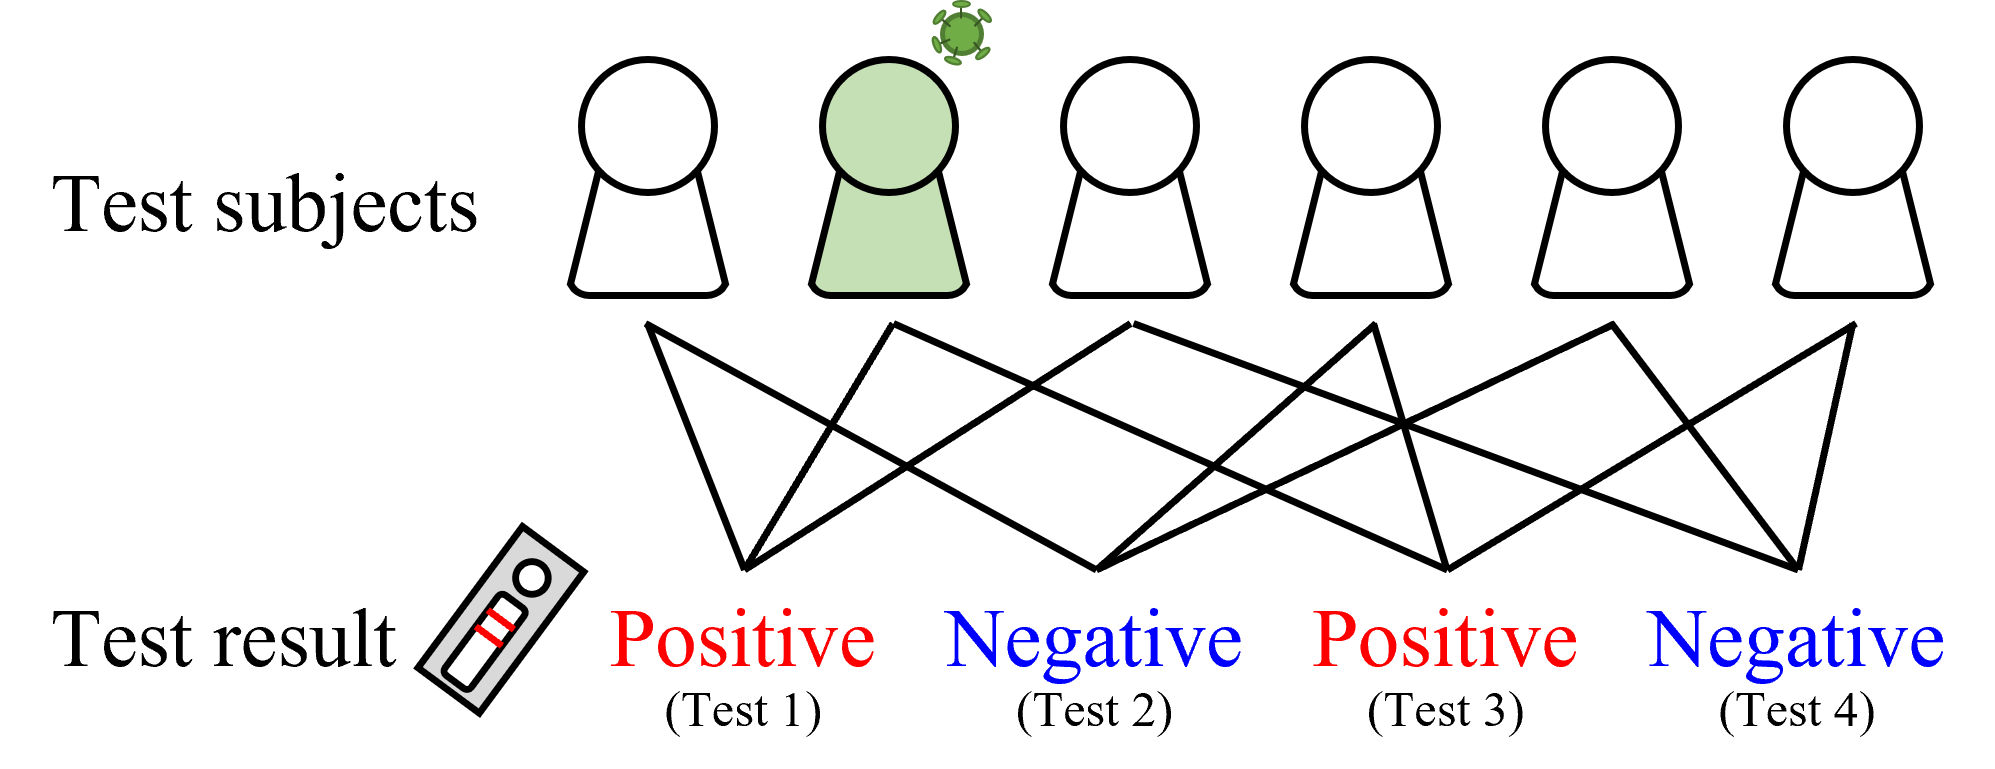
\includegraphics[width=0.6\linewidth]{figures/w11_group_test.png}
    \caption{Group testing. The connected lines show the test subjects sharing a test. The result of a test is negative only if all the people sharing the test is negative (doesn't carry the disease).}
    \label{fig:w11_group_test}
\end{figure}

See the bipartite graph of \autoref{fig:w11_group_test}, we only need $m=4$ tests to determine the infected ones out of $n=6$ people. If a person appears in a negative test, then that person must be negative. The remaining people that cannot be determined are suspicious, and require further testing.

Let us generalize the analysis. Let us use a matrix $A\in\{0,1\}^{m\times n}$ to represent the test schedule, with
\begin{equation}
    A_{ij}:\text{the $i$th test contains the $j$th person.}
\end{equation}
Then we have the result of the $i$th test as
\begin{equation}
    y_i = \bigvee_{j=1}^n (A_{ij} \wedge x_j),
\end{equation}
where $x_j\in\{0,1\}$ is 1 if and only if the $j$th person is infected. The symbol $\vee$ and $\wedge$ represents the logical (boolean) OR and AND operation. As an abuse of notation, one often rewrites the system of equations into the form of $y=Ax$. However, this is by no means a linear algebra problem, it is instead a logic problem.

How do we solve this system of equations to determine $x$?
\begin{example}
    Consider $n=2^5$ and $k=1$, the optimal test is by separating the test subjects into two sets. Consider
    \begin{equation*}
        A = \left[\begin{matrix}
            0 & 0 & 0 & 0 & 0 & 0 & \cdots & 1 \\
            0 & 0 & 0 & 0 & 0 & 0 & \cdots & 1 \\
            0 & 0 & 0 & 0 & 1 & 1 & \cdots & 1 \\
            0 & 0 & 1 & 1 & 0 & 0 & \cdots & 1 \\
            0 & 1 & 0 & 1 & 0 & 1 & \cdots & 1 
        \end{matrix}\right]
    \end{equation*}
    with the $j$th column of $A$ being the binary representation of the number $j$. Then if the $j$th person is infected, i.e. $x_k = \delta_{jk}$, we directly obtain the binary representation of $j$ as $y=Ax$. We only need $m=5$ tests to find the $k=1$ infected person in $n=2^5$ people.
\end{example}

\begin{example}
    \color{red}
    Consider this time $k=2$. For the $j$th column of $A$, let it represent $j$ in its $q$-ary representation ($q=p^n$), for example, $(a_0,a_1,a_2)$. Then we can map $j$ to a polynomial $f(x) = a_0 + a_1x + a_2x^2\in\mathbb{F}_q[x]$. We then evaluate $f$ at $0$, $1$, $\ldots$, $q-1$ and obtain the values $(b_0,b_1,\ldots,b_{q-1})\in\mathbb{F}_q^{q-1}$. We then further turn each $b_i\in\mathbb{F}_q$ into its binary representation, this large vector of 0's and 1's will be the $j$th column of $A$. The decoding then reduces to using the decoding scheme for Reed--Solomon codes.
\end{example}




For more discussions on group testing, please refer to the work by Kautz and Singleton \cite{Kautz_Singleton_64} and \autoref{sec:w12_GT}.